\section{Approach}
%Here what we propose?

%In this project, we intend to use attacks on ADS, to model faults activated in sensors and the communication channels present in an autonomous driving systems. We intend to study the effect of such fault activation (for example, corruption of reported sensor values, corruption of communication channel between sensor and the control system, unexpected activities in hardware controlling the sensor due to faults in control logic etc.) on the output of the entire ADS system.This is an unexplored area and the first step in this research involves formulating of attack models for individual sensors. These attack models will then be used to systematically inject faults in the system and then find vulnerable states in the system.

%We intend to compare the results of this systematic FI with to the existing fault injecting techniques and compare the performance and accuracy of these system by answering following questions. 

%\begin{itemize}
%\item  Does employing systematic approach to FI increase the performance in comparison to fuzz testing?

%\item Does benefit obtained in terms of performance justify the effort required for developing systematic approaches for FI?

%\end{itemize}
%The information collected using these individual attack models will then be used to find the vulnerabilities in the integrated ADS system. To detect and provide resilience against detected vulnerabilities, we will develop a model-based analysis framework, based on the dynamics of the ADS in order to test for any behavior not corresponding to system specifications.

%We propose development of a systematic method to find vulnerabilities in components of an ADS, instead of using standard ad-hoc approaches~\cite{jha18dsn}~\cite{jha18art}, which don't provide good coverage for resilience assessment. The main objective of this project will be to develop a technique that can detect all vulnerabilities in sub-components that lead to degradation of reliability of whole system. This is an unexplored area and the first question in this research will be to find out, if this method is feasible. This involves formulating of fault models for individual components of an ADS. After development of fault models, individual components will be manually tested for vulnerabilities to test the validity of these fault models. This testing will be generalized and automated later by developing a tool that systematically finds all the vulnerabilities specified by the fault model of a component. The information collected using these individual fault models will then be used to find the vulnerabilities in the integrated ADS system and improve its resilience.

%CARLA will be used as a test platform for development and testing of our approach as it provides a convenient way to instrument and modify the readings of different sensors, as well as the behavior of driver agents that controls the autonomous vehicle. 

%Current approaches that analyze resilience of ADS systems on a holistic level perform fault injections to find vulnerabilities in the system which is quite resource intensive. Details about such approaches is provided in section \ref{related_work}. Our proposed methodology will forgo such ad hoc approaches and test different components of an ADS in a systematic way by modeling its behavior and using formal methods to validate its correctness and finding any unexpected behavior that introduces vulnerabilities in the ADS system. 
 \begin{figure*}
 	\centering
 	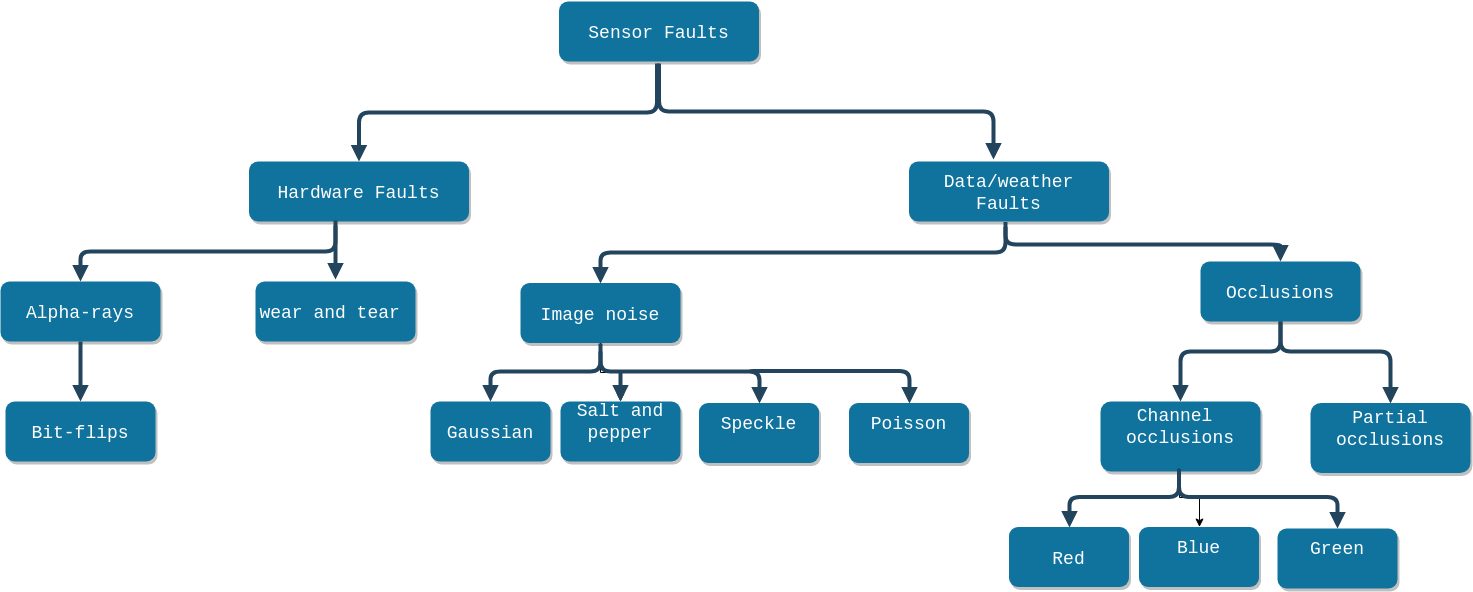
\includegraphics[width=0.7\linewidth]{finalFM}
 	\caption[Fault model for camera]{}
 	\label{fig:finalfm}
 \end{figure*}
 


% Our contribution
Our contribution is two-fold in this work. First, by an in depth understanding of autonomous vehicles, we device a fault model for the vehicle in general. We specifically focus on the sensor faults and design a fault-model specific to the sensors. Second, based on our fault model, we inject faults in order to obtain the failure rate of the system caused due to the sensor faults. We attempt fault injection in order to get maximum coverage of the system in an optimal manner.

\subsection{Fault-model for ADS}
% general categorization of the fault-model
Analyzing the system, we designed a fault model for autonomous driving systems. We categorized the fault occurrence in two ways: due to some physical damage or due to network issues. These two categories of faults cover almost all possible components of the systems which can lead to a failure of the system. 

%\\TODO- components of the LIDAR.





%why do we define the fault-model of the entire system
In Figure~\ref{fig:fault-modelgeneral} we provide a fault-model for an ADS. However, covering the failures caused by each component is out of scope of our current paper. Also, analysing failure rates in general instead of component wise failure rates does not provide us with useful set of results. Hence we introduce a fault-model for the sensors of an ADS. 

%Core Components we selected for faults in ADS
 The core component we selected were the  sensors used in ADS. The sensors are one of the most expensive parts of an ADS. Hence, determining the failure rates due to these sensors can help us in minimizing damage. We described different categories of sensors in Section-3. We start with an analysis of one of the sensors described above.
 
 \subsection{Fault-model of Camera}
 %A little more about Camera
 Camera is a very expensive sensor and hence finding the failure rates of the system, caused due to camera can help the designers understand how to mitigate the faults such that they don't lead to failures. ADS being safety critical systems, can cause a lot of harm ( death in the worst case scenario ) in case of a failure. 
 
 \subsubsection{Hardware faults} These faults represent the soft errors that can occur in the data, that is recorded by the sensors. These faults can occur in the registers of sensor units or in communication links between sensor and controller. These faults can also occur within registers, where these values are stored in the main ADS controller. In our study we  assume that the fault is always activated regardless of where the fault actually occurred. This manifests in the form of sensor data being altered before it is used by controller to make decisions. These type of faults in real life can introduce single bit-flips which is modeled by our fault model. 

 %introduce the notion of 
 We created two categories of faults under this section. The first is due to the alpha-rays which causes random bit flips. The other set of faults which can occur is due to wear and tear of the sensor. Sometimes, buying cheaper sensors can lead to a faster wearing away of sensors. 
 \medskip
 \subsubsection{Data Faults} These faults refers to the conditions in which the sensors give readings which are not correct representation of the environment. These faults can occur due to manufacturing defects in the sensors and various environmental conditions. Environmental conditions can refer to weather and other characteristics of the environments that are used in decision making process by the ADS.. For example, A camera mapping its surroundings can be effected by rainy weather or intense monochromatic lights, which may lead to addition of noise in the image captured by the camera sensor.
 
 \subsection{CARLA} \label{ri-carla}
 CARLA is an open source simulator which simulates a dynamic world and provides a simple interface between environment and autonomous vehicles (AV). The simulation engine simulates a vehicle in a city environment with realistic physics. Measurements representing the environment are provided to a driving agent (DA) which  controls the actions that the AV takes based on these measurements and some predefined algorithm. Figure~\ref{fig:carla_arch} shows the high level architecture of CARLA. CARLA operates in a server-client model in which server handles the simulations, while client controls the actions of the AV(through DA) as well as simulation parameters of the overall system. 
 %\subsubsection{Client} It runs the simulation and renders the environment that the AV experiences.
 
 %\subsubsection{Server} It controls the parameters of the simulation and also controls the actions of the AV based on predefined algorithms. 
 
 \begin{figure}  [h]
 	\vspace{-0.5em}
 	\centering
 	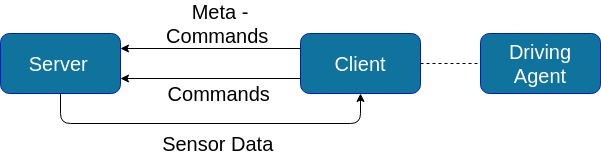
\includegraphics[scale=0.4]{CARLA_block}
 	\vspace{-0.5em}
 	\caption{High level architecture of CARLA, Server sends sensor data to the client which integrates with driving agent and returns driving commands to server.}
 	\label{fig:carla_arch}
 	\vspace{-1.5em}
 \end{figure}
 
 \bigskip
 
 %Due to this client-server architecture CARLA provides flexibility to swap multiple driving algorithms (called driving agents in CARLA terminology) and driving environments easily. The server provides the ability to render a range of environments by changing the weather, number of vehicles and pedestrians etc in the simulation environment. The server also provides the output of various sensors attached to AV to the driving agent. The client connects to the server using sockets and provides two type of inputs, commands and meta-commands, to the server. Commands control the behavior of the vehicles i.e braking, steering, accelerating etc. and are provided by the driving agent which is integrated with client side in CARLA using python APIs. Meta-commands are used to control the behavior of simulation.
 
 Although CARLA provides ability to simulate complex environments, Dosovitskiy et al.~\cite{Dosovitskiy17} have shown that for a range of driving agents, only simple paths with no dynamic actors produce successful results for more than ninety percent of trials.
 
 \medskip
 
 \subsubsection{Driving Agent}
 As mentioned in the previous section the behavior of the vehicle in the simulation is controlled by the driving agent. Our goal is to study the resilience of ADS in CARLA, so we have chosen a driving agent developed by Codevilla et al.~\cite{Codevilla2018}, which uses conditional imitation learning to train a recurrent deep neural network. This network is used in simulation for selecting appropriate action based on sensor. Dosovitskiy et al.~\cite{Dosovitskiy17} tested multiple driving agents and have shown that success rate of imitation learning based driving agent is highest(~90\%). Table~\ref{table:1} shows the results of this study for our testing conditions.
 
\begin{table}
	\begin{tabular}{| c | c | c | c |}
		\hline
		Drving agent & Training env. & Testing env. & Average  \\
		\hline
		Multi-layer perceptron & 82 & 95 & 88.5  \\ 
 		Imitation Learning & 89 & 90 & 89.5 \\  
 		Reinforcement Learning  & 34 & 16 & 25 \\
 		\hline
 	\end{tabular}
 \caption{Percentage of successful episode for different driving agents~\cite{Dosovitskiy17}.}
 \label{table:1}
\end{table}

 \medskip

 %The fault space for even one sensor using approach mentioned above is quite big, which may lead to state space explosion. We intend to use this approach as a stepping stone towards finding a systematic approach for FI.  
 
 \subsubsection{Environment Setup}
 \setcounter{subsubsection}{0}
 In our study we focus on the sensor faults, so to avoid skewing of results due to any machine learning error we select a subset of paths for fault injections, in which the ADS encounters no machine learning errors and is always able to complete the predefined goal without any traffic violations in all weather conditions.  
 \medskip
 \begin{itemize}
 	\item \textbf{Path:} Length of the paths selected for our experiments ranges from 70 to 100 meters and contains one turn between the starting and the ending position. 
 	
 	\smallskip
 	
 	\item \textbf{Environment:} No dynamic objects (i.e. NPC vehicles, pedestrians etc.) are present in the simulation environment and six predefined weather conditions provided by CARLA are used for each path. 
 \end{itemize}
 
 \subsection{Fault Injection} \label{fi_m}
 
 In our study with random Fault injection we study each fault separately, so for a set of related experiments we only inject one type of fault. A single fault is injected, according to the fault model, in each execution run and its effect on the overall system is observed. The objective and path to navigate is constant in each trial so that its outcome can be compared with output of a golden run, in which no fault was injected. 
 
 %\textcolor{red}{We need a text block about how we represent different faults and justify it, from literature review}
 The output of optical sensor in attached to ADS used for experiments, is a three dimensional array of size 600 x 800 x 3, which represents an RGB image of size 600 x 800. The value for each pixel ranges from 0 to 255 for all channels. The fault in the camera sensor can be simulated by altering the captured image. For example, partial occlusion fault in the experiments is simulated by selecting a random portion of the image of size 100 x 200 and setting the value of all the pixels in this portion to 0. Figure~\ref{fig:partial_occlusion} shows the effect of partial occlusion on the sensor data. Details about effect of other faults are mentioned in Appendix~\ref{Appendix:A}.
 
 \begin{figure}[h]
 	\vspace{-0.5em}
 	\centering
 	\begin{subfigure}[b]{0.23\textwidth}
 		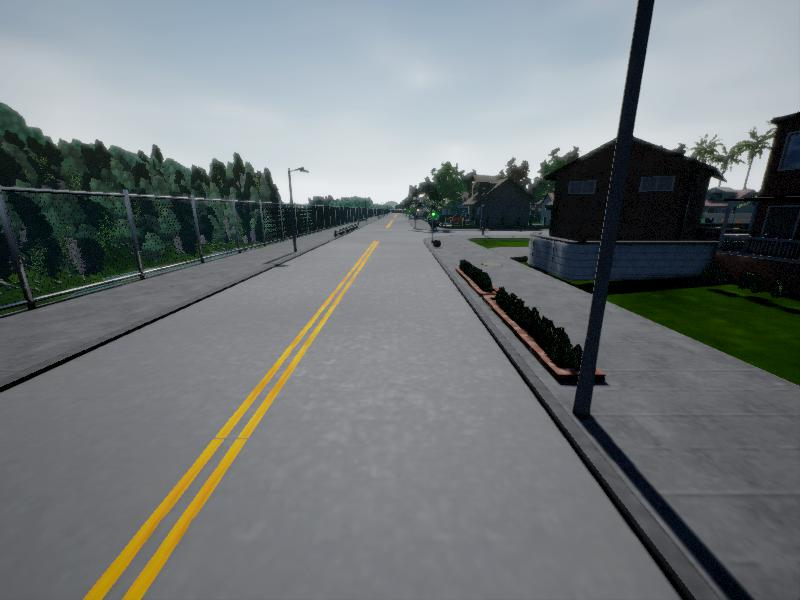
\includegraphics[scale=0.15]{pure_data}
 		\caption{Sensor output}
 		\label{fig:fs_example}
 	\end{subfigure}
 	~ 
 	\begin{subfigure}[b]{0.23\textwidth}
 		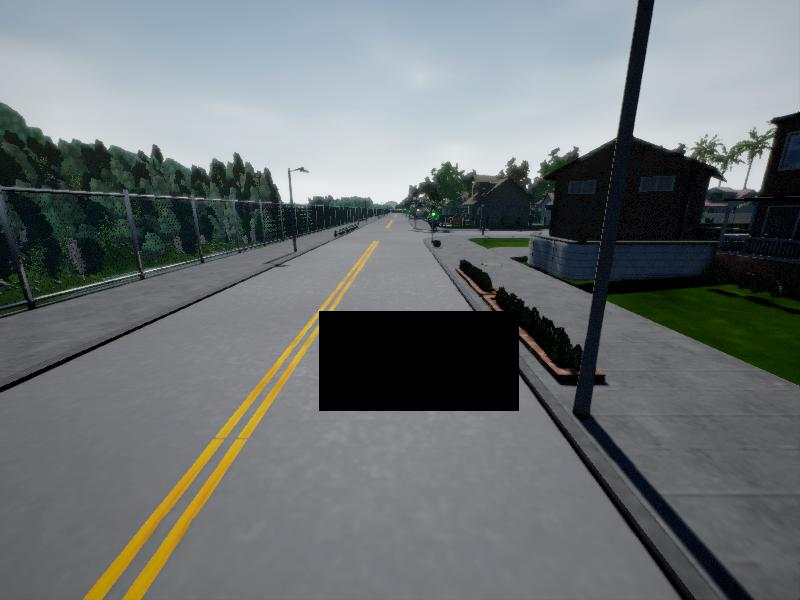
\includegraphics[scale=0.15]{faulty_data}
 		\caption{Sensor output after FI}
 		\label{fig:fc_example}
 	\end{subfigure}
 	
 	%\vspace{-1em}
 	\caption{Effect of partial occlusion fault}
 	\label{fig:partial_occlusion}
 	\vspace{1.5em}
 \end{figure}
 
 As mentioned in~\ref{ri-carla} CARLA provides a client server architecture. We exploit this boundary between client and server for our fault injection experiments. Figure~\ref{fig:FI_method} provides an overview of FI method used in one trial. CARLA platform provides an ability to run multiple trials of the same experiments (same environment and goals). Each trial involves multiple steps. In each step, data is read from the sensors, which is provided to the driving agent, which based on some predefined algorithm, gives command to the AV, after the command, it is checked if the objective of the trial is achieved or a timeout has happened. If any of these condition exists, we end the current trial and the using the measurements from the server, the metrics defined in~\ref{fi_m} are calculated for this trial.
 
 \begin{figure}  
 	\vspace{-0.5em}
 	\centering
 	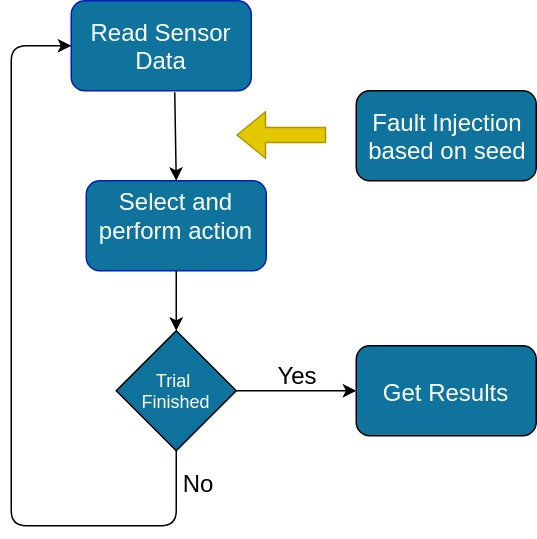
\includegraphics[scale=0.3]{FI_method}
 	\vspace{-0.5em}
 	\caption{Life cycle of an experiment trial on client side, Fault is injected by altering sensor readings received by client.}
 	\label{fig:FI_method}
 	\vspace{-1.5em}
 \end{figure}
 
 The sensor readings are provided in form of dictionary to driving agent from the client, which can be easily accessed in the code. We insert a code block in between reading data from server and sending it to driving agent. This code block changes the reading of the sensor under study, based on the fault under consideration.
 
 We use the following metrics to quantify the resilience of ADS which are inline with previous work in this domain~\cite{avfi}.
 \setcounter{subsubsection}{0}
 
 \medskip
 \subsubsection{Success percentage} This metric represents the fraction of total trials in which the ADS was successful in completing its objective i.e. navigate successfully from starting position to end point with in specified time.
 
 \smallskip
 
 \subsubsection{Success percentage without violations} This metric captures the traffic violations that occur during each trial. This is a more stricter criteria which records trials with no violations. The violations that we consider for calculating this metric are lane violation, curb violations and traffic law violations (reasons for not considering collisions with dynamic objects are explained in \ref{ri-carla}). 
 
 The two metrics used, provide and opportunity to study the effects of faults on the overall functioning of AV as well as the lower level deviations from normal behavior, which may not lead to outright failure but violate safety properties.
 